\section{Bài 1:}
\begin{enumerate}
\bf
\item Sử dụng mô hình cho sẵn (đính kèm trong tập tin Project3{\_}1.pkt) để trả lời các yêu cầu bên dưới:

\rm Điền thông tin còn thiếu vào bảng: (các ô không có dấu -):

Các thông tin còn thiếu được điền bằng màu xanh.
\begin{table}[H]
\begin{center}
\begin{tabular}{|c|c|c|c|c|}
\hline
\textbf{Device}&\textbf{Interface}&\textbf{IP address}&\textbf{Subnet mask}&\textbf{Default gateway}\\
\hline
Router0&G0/0&\textcolor{blue}{192.168.1.1}&\textcolor{blue}{255.255.255.0}&-\\
\hline
Router0&G0/1&\textcolor{blue}{192.168.8.1}&\textcolor{blue}{255.255.255.0}&-\\
\hline
Router1&G1/0&\textcolor{blue}{192.168.2.1}&\textcolor{blue}{255.255.255.0}&-\\
\hline
Router1&G1/1&\textcolor{blue}{192.168.8.2}&\textcolor{blue}{255.255.255.0}&-\\
\hline
PC0 (PC1 trên hình \ref{fig1.1})&-&\textcolor{blue}{192.168.1.10}&\textcolor{blue}{255.255.255.0}&\textcolor{blue}{192.168.1.1}\\
\hline
PC1 (PC2 trên hình \ref{fig1.1})&-&\textcolor{blue}{192.168.2.10}&\textcolor{blue}{255.255.255.0}&\textcolor{blue}{192.168.2.1}\\
\hline
\end{tabular}
\caption{Điền thông tin còn thiếu}
\end{center}
\end{table}


\begin{figure}[H]
\begin{center}
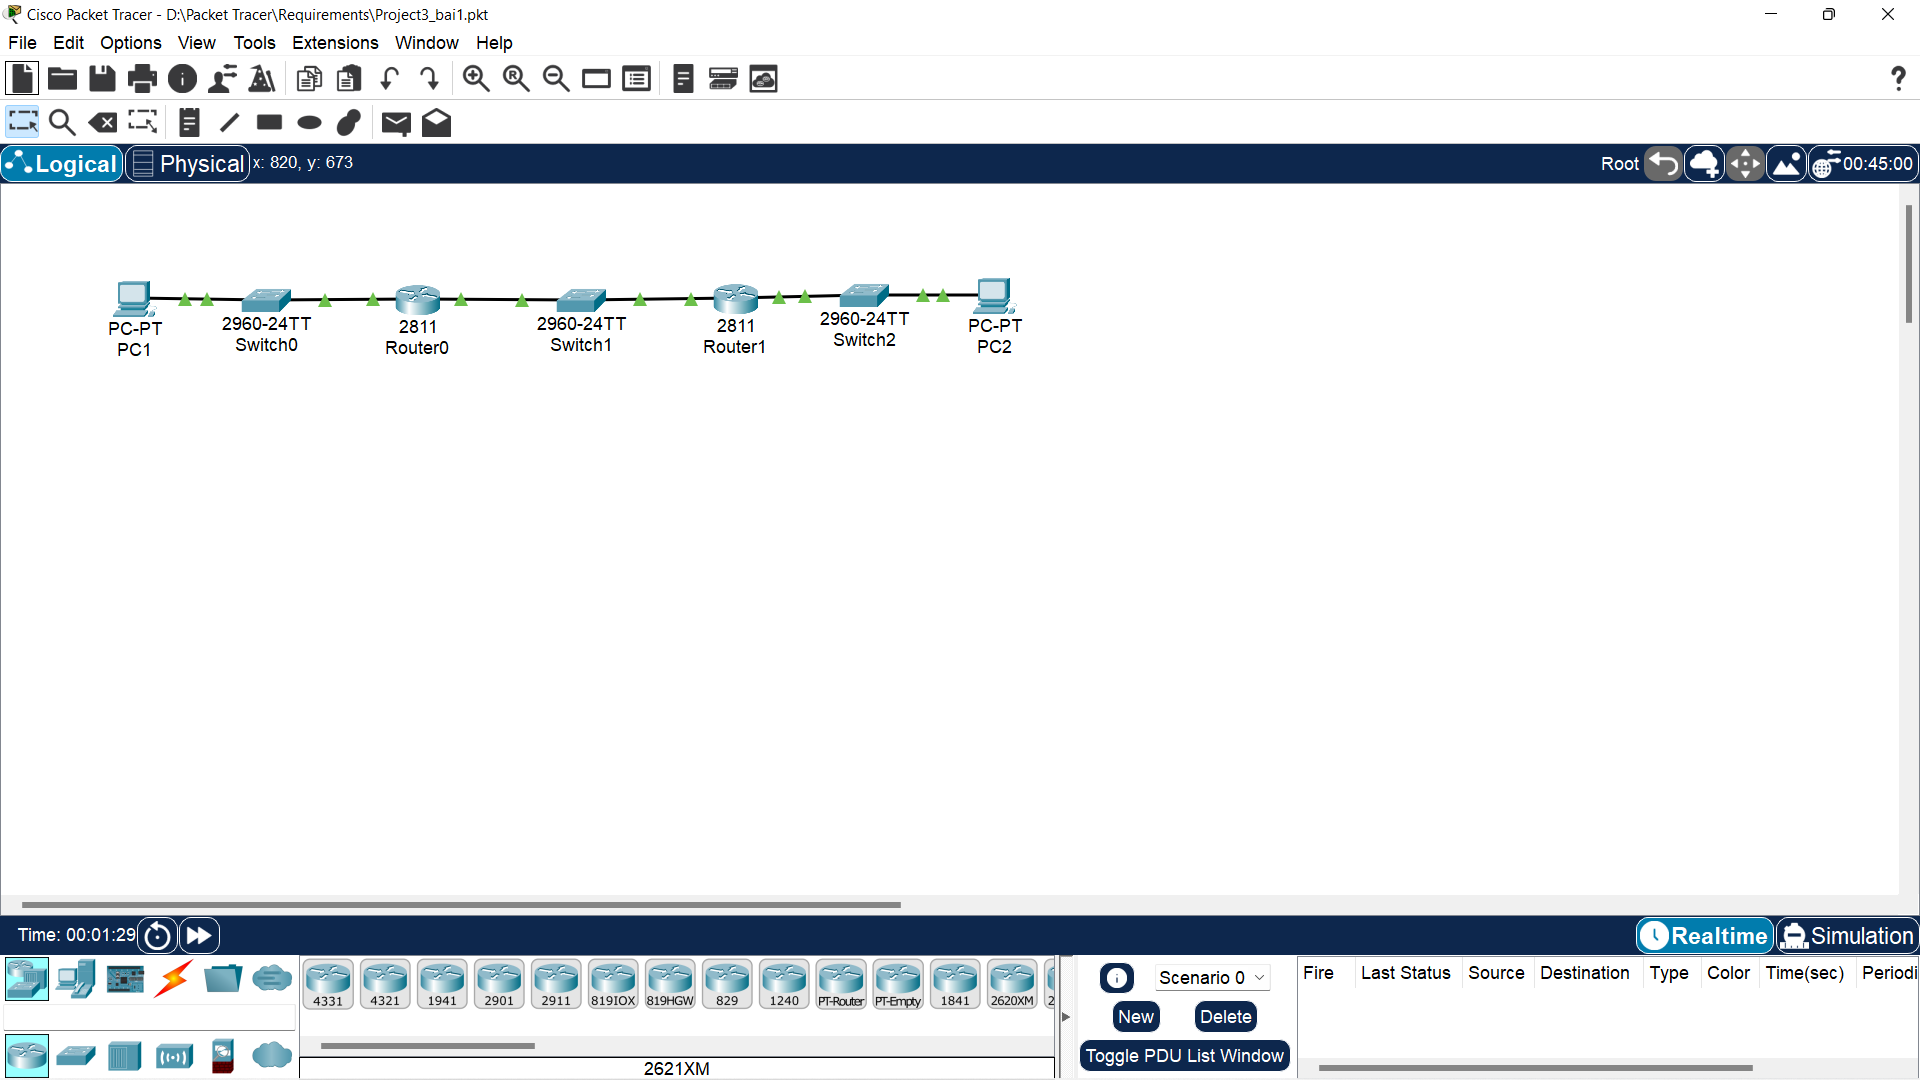
\includegraphics[scale=0.5]{../figures/p1/p1-prob}
\end{center}
\caption{Nội dung tập tin Project3{\_}1.pkt ban đầu}
\label{fig1.1}
\end{figure}

\begin{figure}[H]
\begin{center}
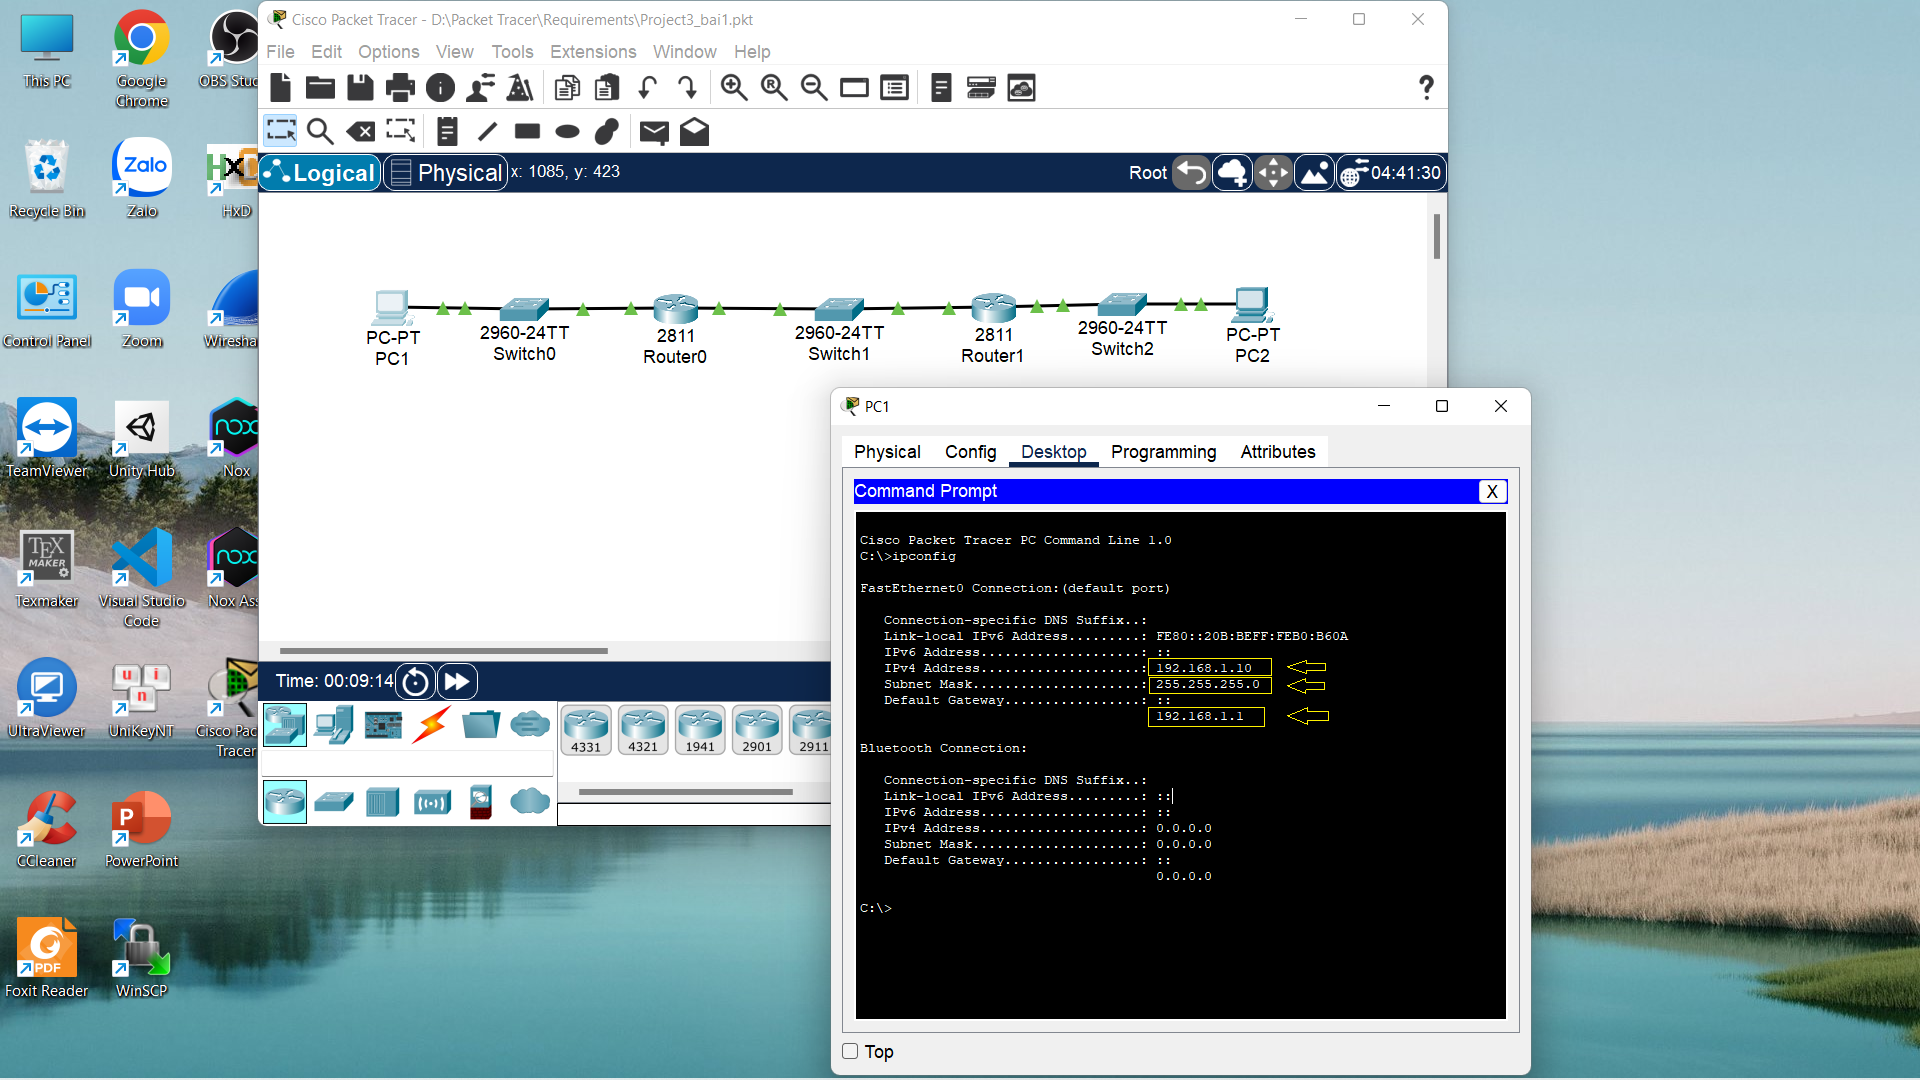
\includegraphics[scale=0.5]{../figures/p1/p1-ipconfig-pc}
\end{center}
\caption{Kiểm tra thông tin IP của PC}
\end{figure}

\begin{figure}[H]
\begin{center}
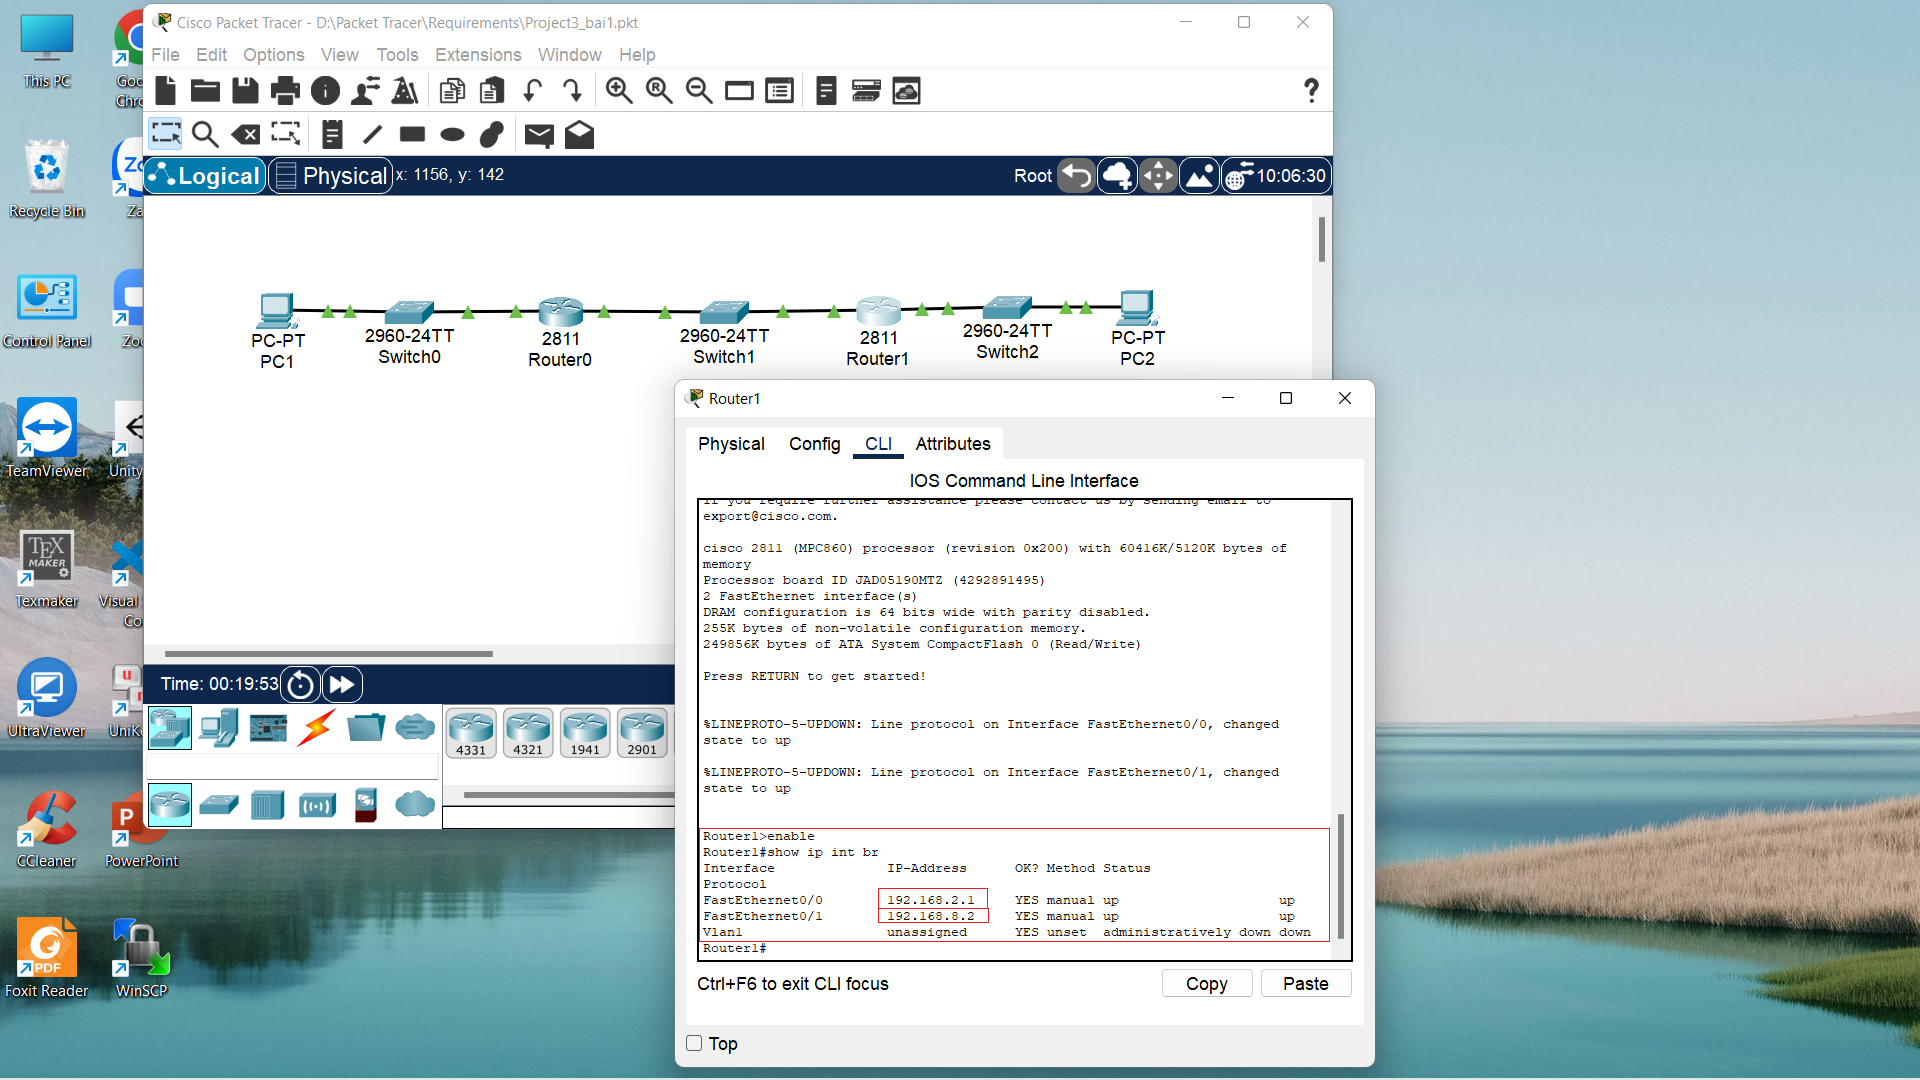
\includegraphics[scale=0.5]{../figures/p1/p1-ipconfig-router}
\end{center}
\caption{Kiểm tra thông tin IP của router}
\end{figure}

\bf \item Ghi chú đầy đủ các thông tin interface, địa chỉ đường mạng, địa chỉ IP lên mô hình mạng:

\rm 
\begin{figure}[H]
\begin{center}
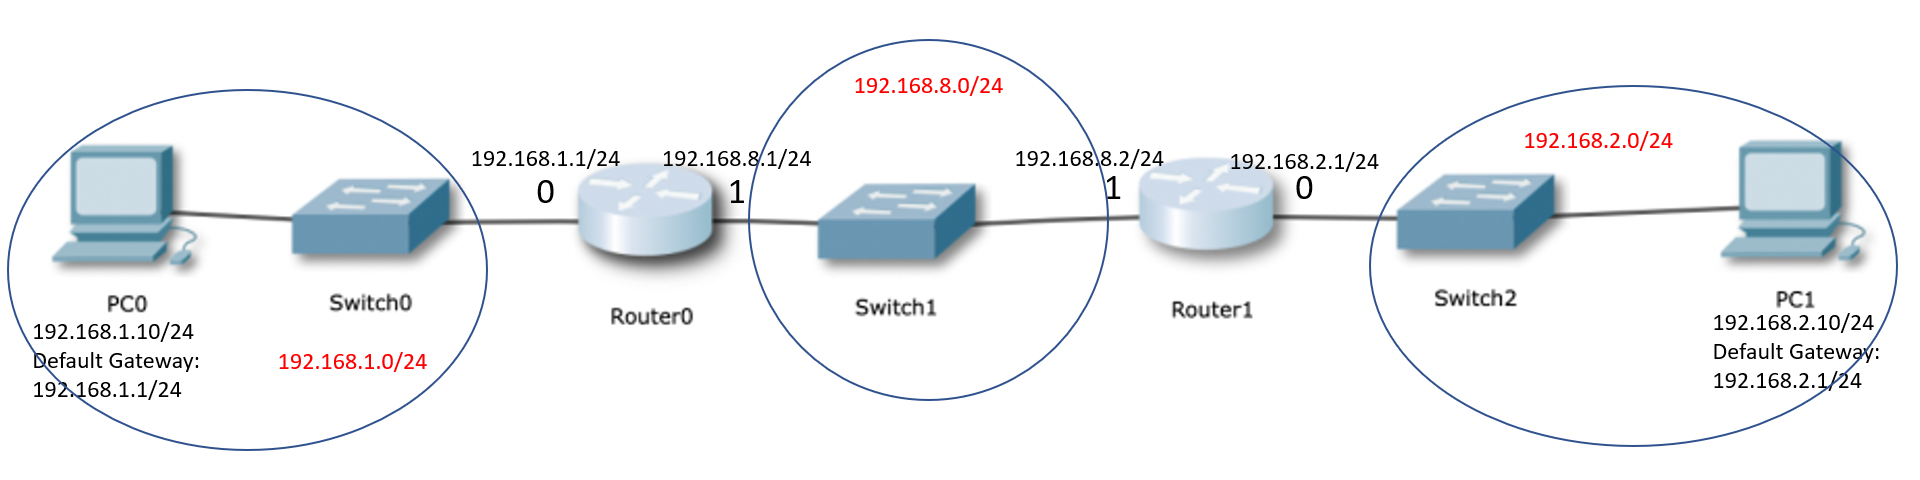
\includegraphics[scale=0.5]{../figures/p1/p1-2}
\end{center}
\caption{Mô hình mạng}
\end{figure}

\bf \item Hãy cho biết các router có được cấu hình gateway hay không? Nếu có hãy viết thông tin gateway của từng router.

\rm Cả 2 router đều chưa được cấu hình gateway.

\begin{figure}[H]
\begin{center}
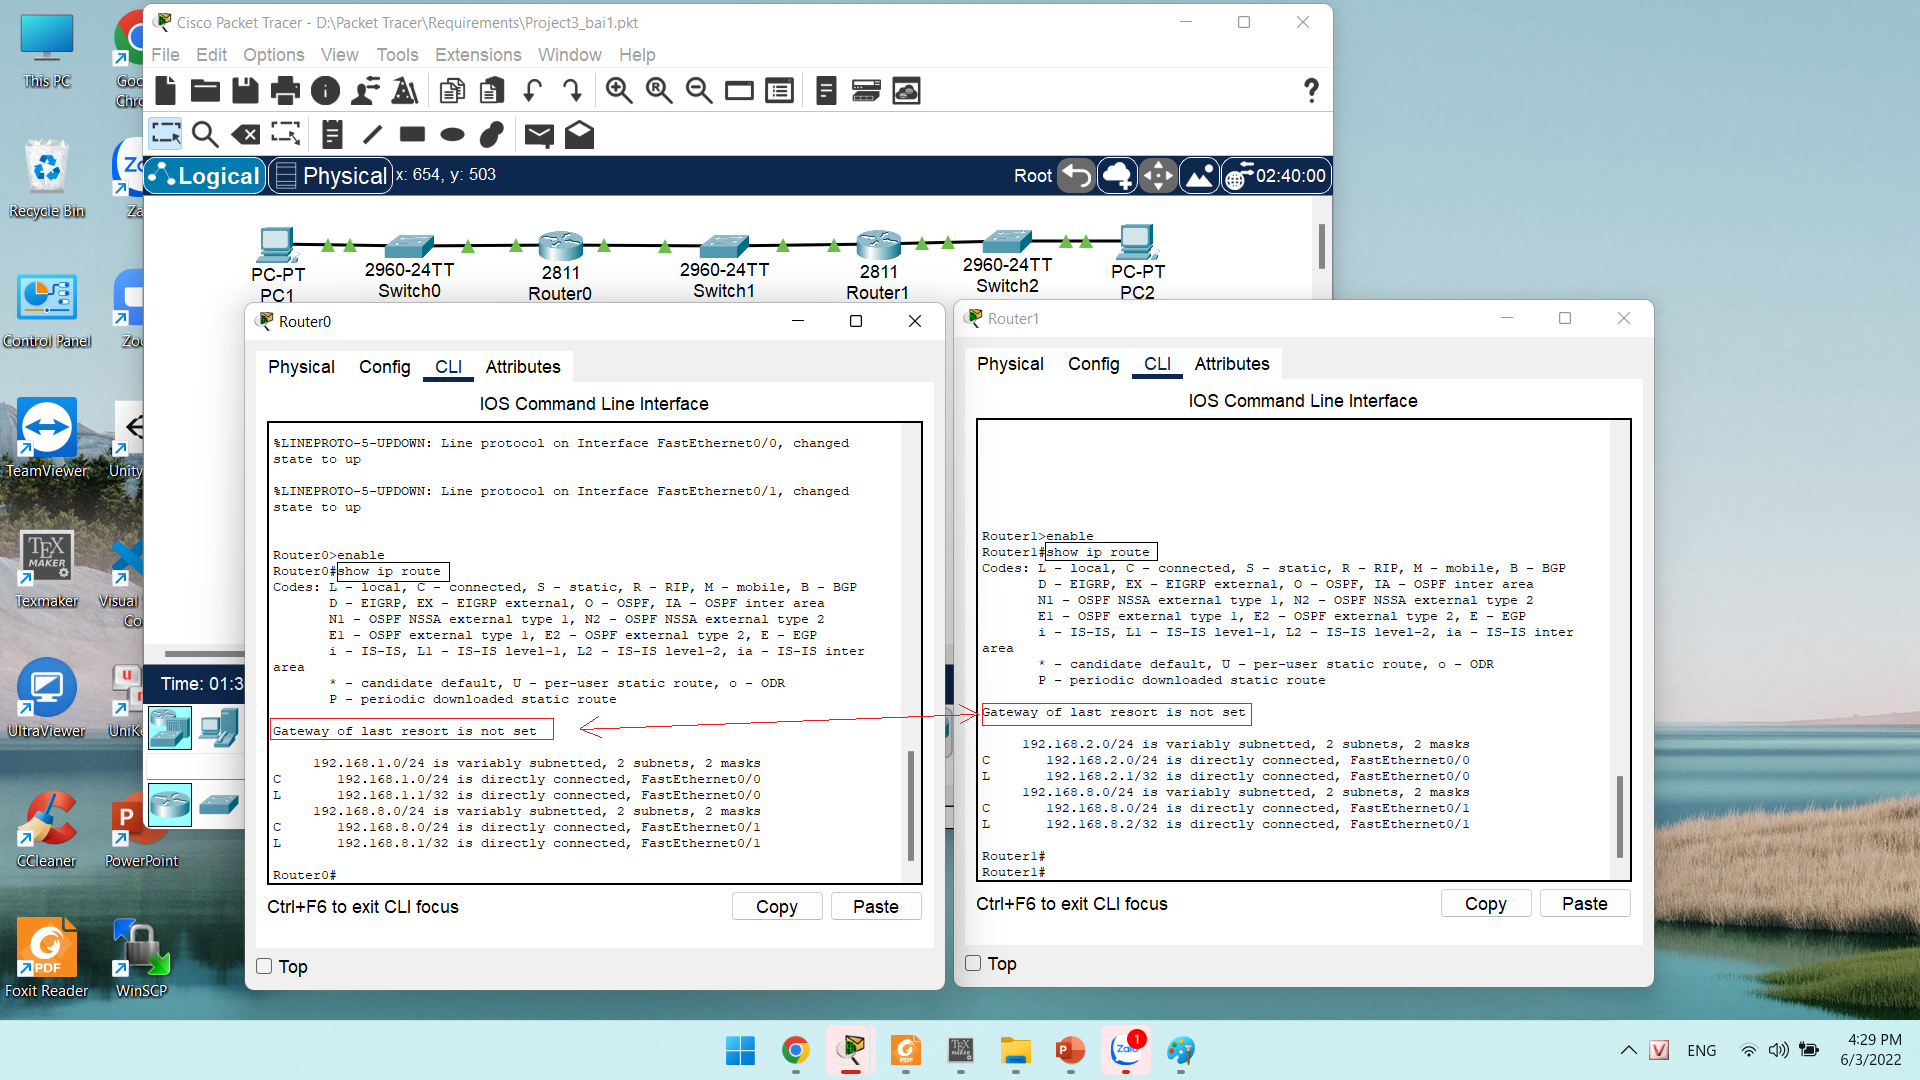
\includegraphics[scale=0.5]{../figures/p1/p1-3}
\end{center}
\caption{Kiểm tra cấu hình gateway}
\end{figure}

\bf \item Kiểm tra kết nối từ PC0 đến PC1, cho biết kết quả như thế nào? (ở lần ping đầu tiên các gói tin ICMP có được gửi thành công hay không). Cho biết đường đi của gói tin ICMP (đi qua các thiết bị, IP nào?)

\rm 

\begin{figure}[H]
\begin{center}
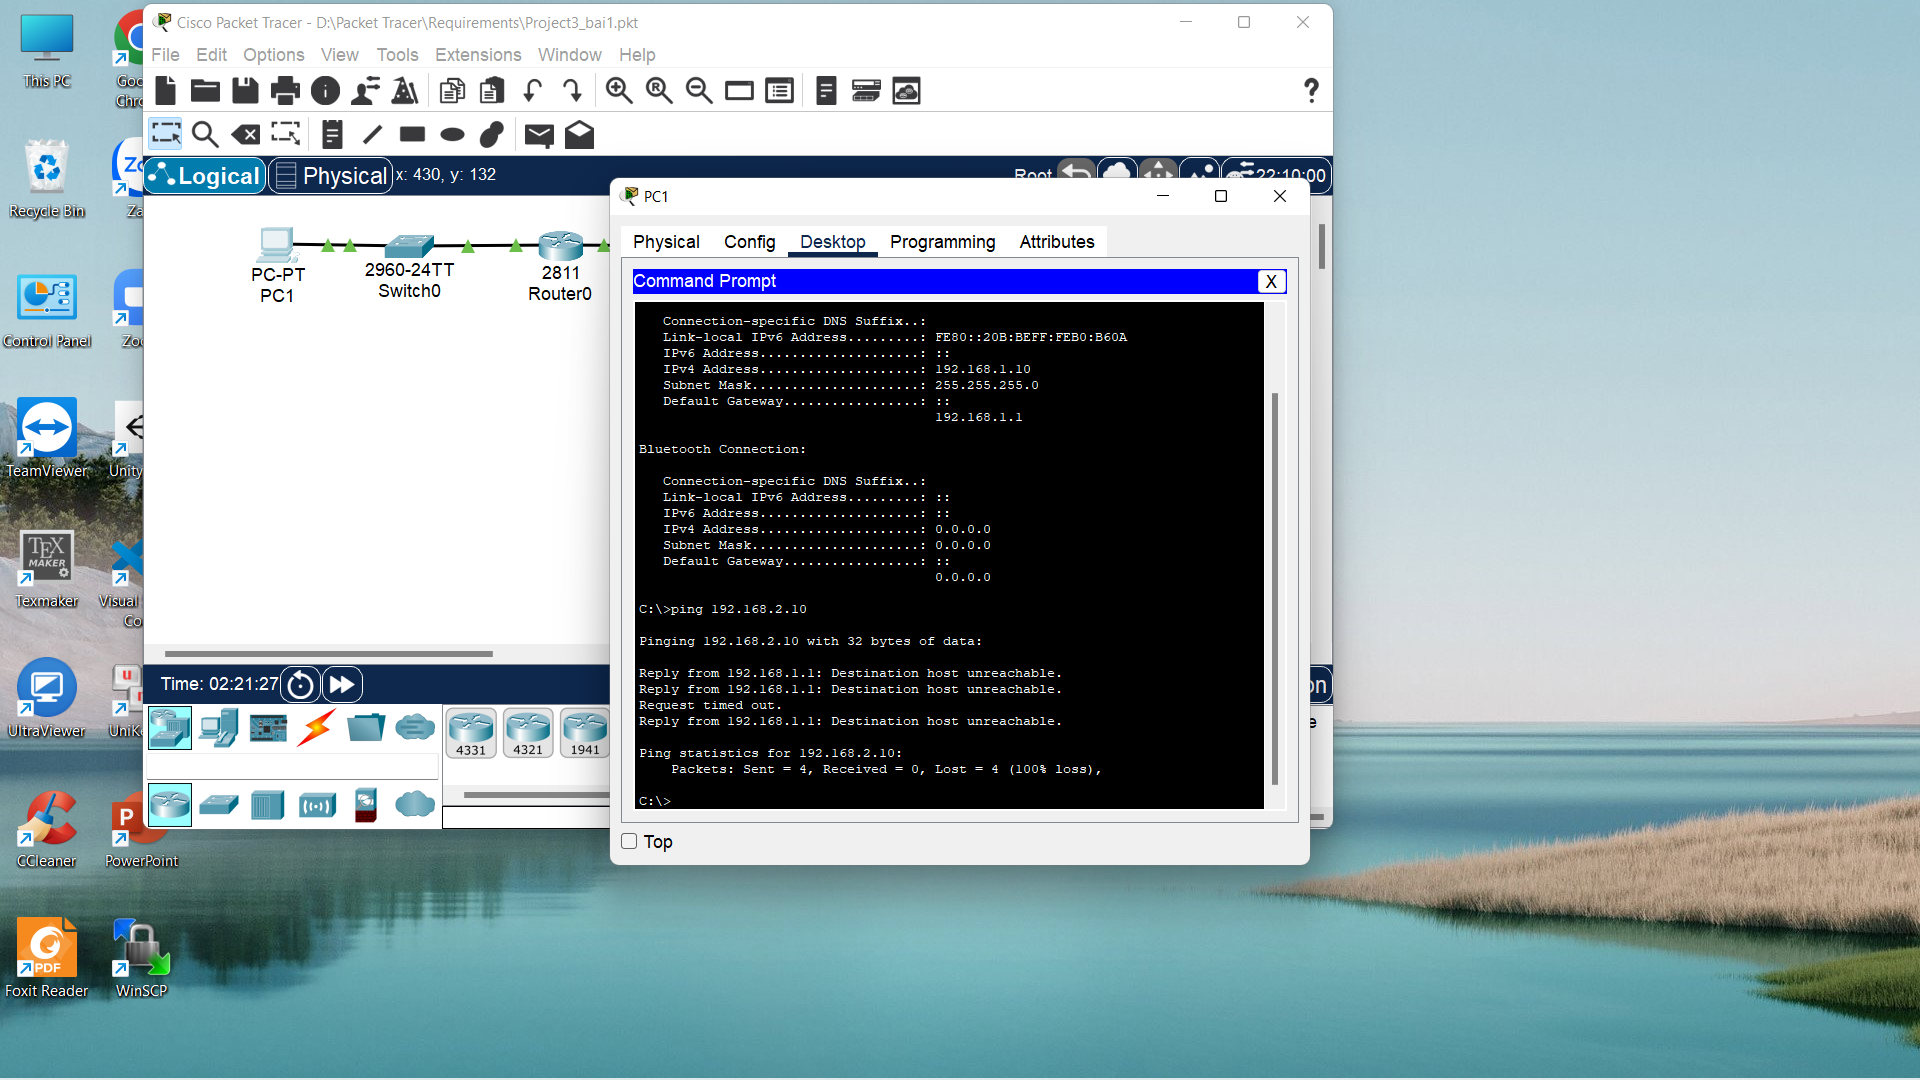
\includegraphics[scale=0.5]{../figures/p1/p1-4}
\end{center}
\caption{Kiểm tra kết nối từ PC0 (\texttt{192.168.1.10}) đến PC1 (\texttt{192.168.2.10})}
\end{figure}

Lúc này cả 2 router chưa cấu hình thông tin định tuyến, do đó máy PC0 trong mạng \texttt{192.168.1.0/24} chưa thể kết nối với máy PC2 trong mạng \texttt{192.168.8.0/24}. Gói tin chỉ đến được router0 cổng 0 (192.168.1.1).

\bf \item Thêm PC2 vào đường mạng \texttt{192.168.8.0/24}. Cấu hình địa chỉ IP, subnetmask, gateway tương ứng cho PC2.

\rm

\begin{figure}[H]
\begin{center}
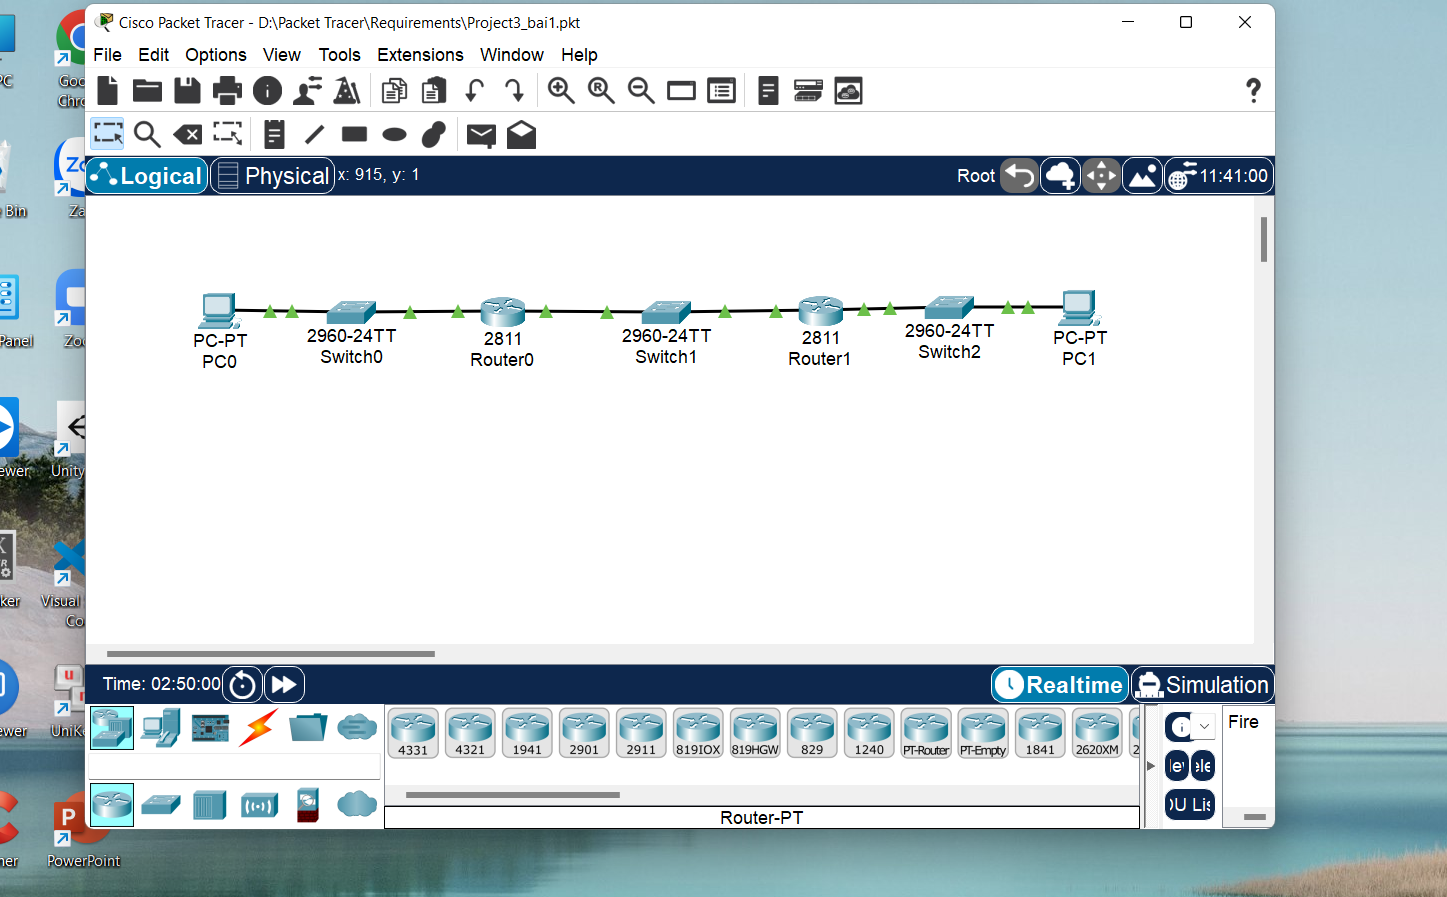
\includegraphics[scale=0.5]{../figures/p1/p1-5a}
\end{center}
\caption{Trước khi thêm PC2}
\end{figure}

\begin{figure}[H]
\begin{center}
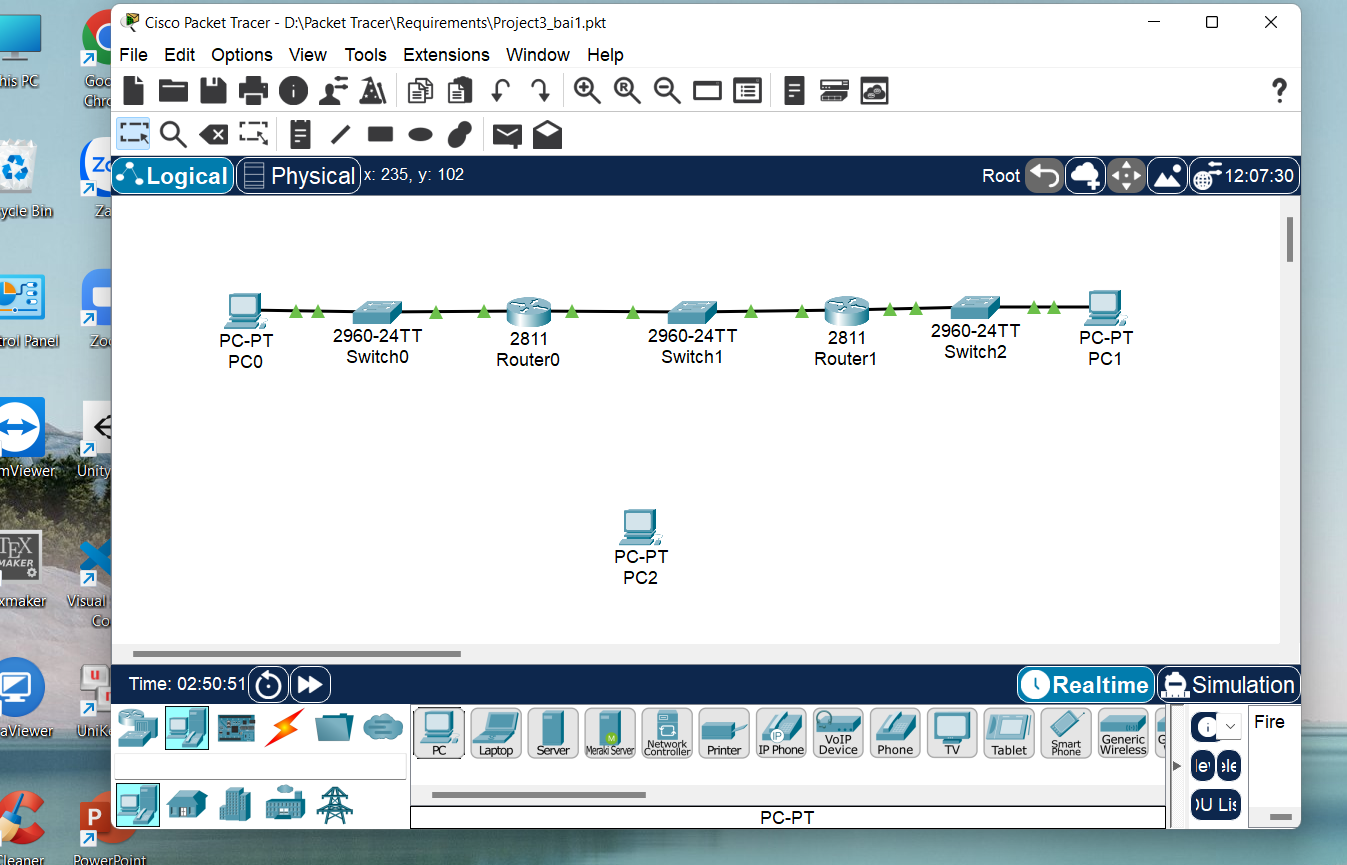
\includegraphics[scale=0.5]{../figures/p1/p1-5b}
\end{center}
\caption{Thêm máy tính mới PC2}
\end{figure}

\begin{figure}[H]
\begin{center}
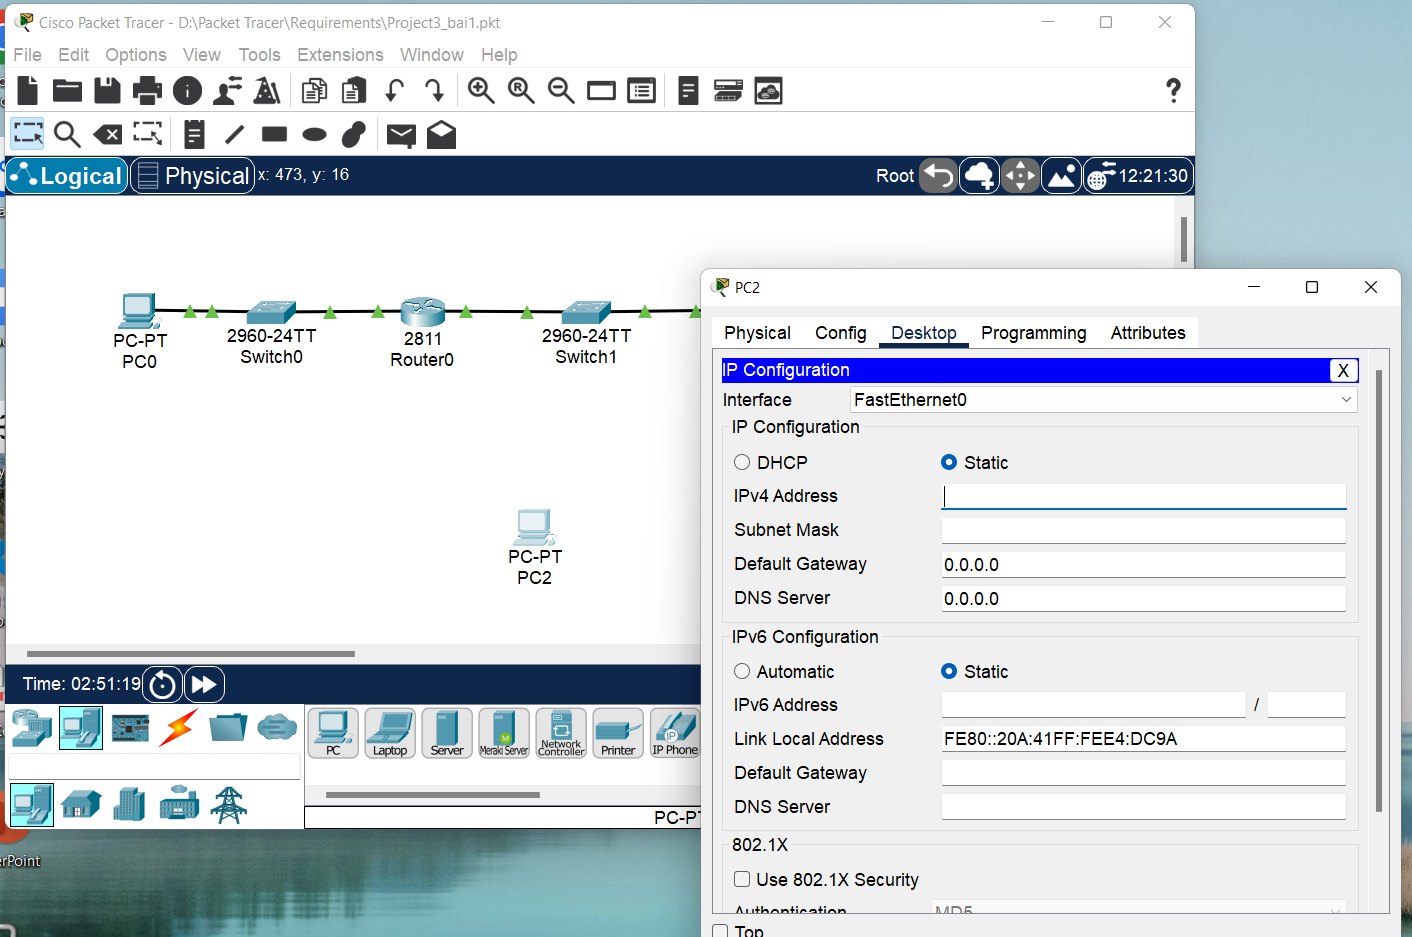
\includegraphics[scale=0.5]{../figures/p1/p1-5c}
\end{center}
\caption{Mở cấu hình máy}
\end{figure}

\begin{figure}[H]
\begin{center}
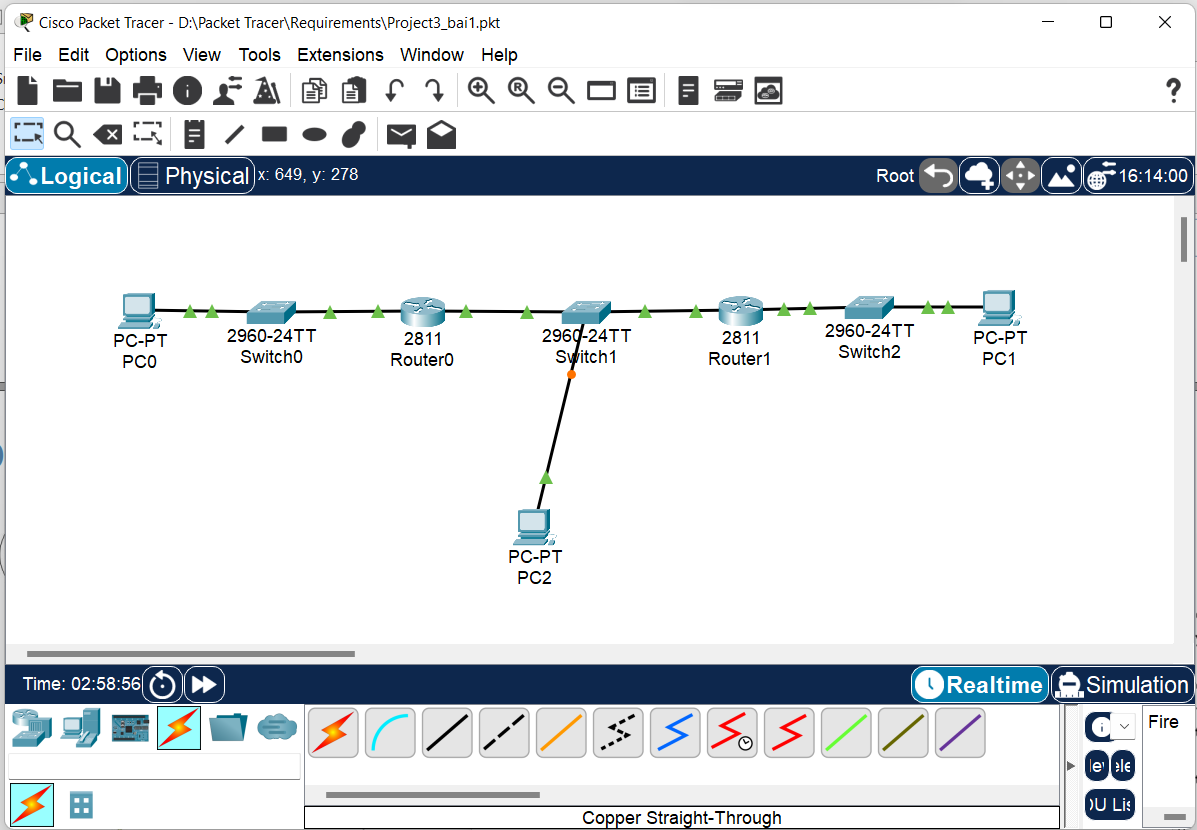
\includegraphics[scale=0.5]{../figures/p1/p1-5d}
\end{center}
\caption{Nối PC2 với Switch1 (Switch1 đang nối 2 router với các cổng \texttt{192.168.8.1} (của Router0), \texttt{192.168.8.2} (của Router1))}
\end{figure}

\begin{figure}[H]
\begin{center}
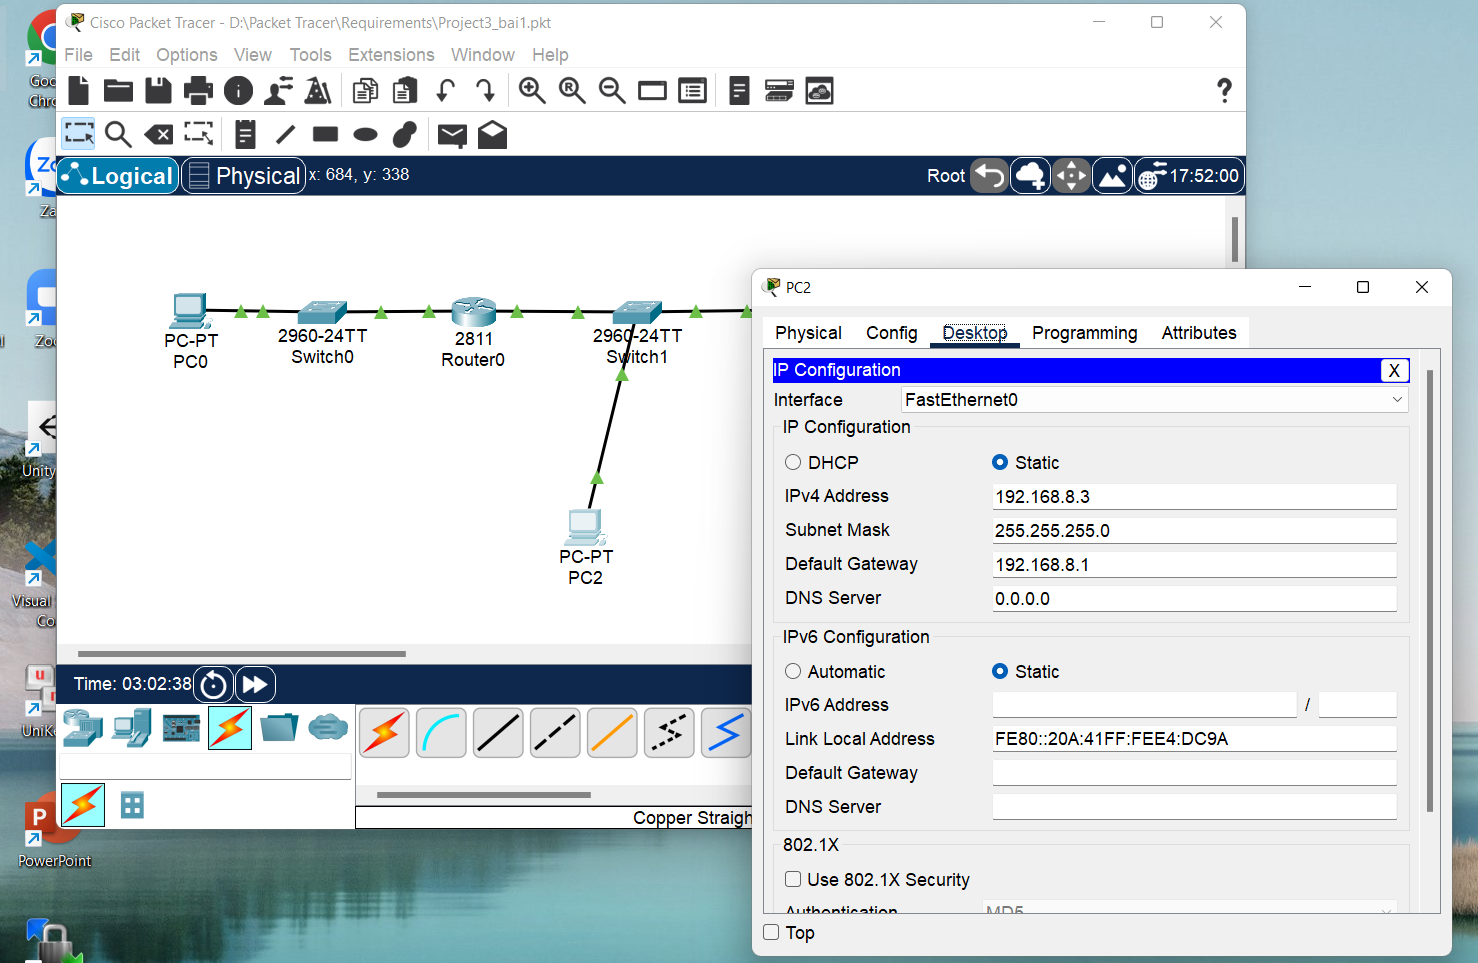
\includegraphics[scale=0.5]{../figures/p1/p1-5e}
\end{center}
\caption{Cấu hình máy PC2, chọn default gateway là \texttt{192.168.8.1}}
\end{figure}


\bf \item Kiểm tra kết nối từ PC0 đến PC2, cho biết kết quả như thế nào? (ở lần ping đầu tiên các gói tin ICMP có được gửi thành công hay không). Cho biết đường đi của gói tin ICMP (đi qua các thiết bị, IP nào?)

\rm 
\begin{figure}[H]
\begin{center}
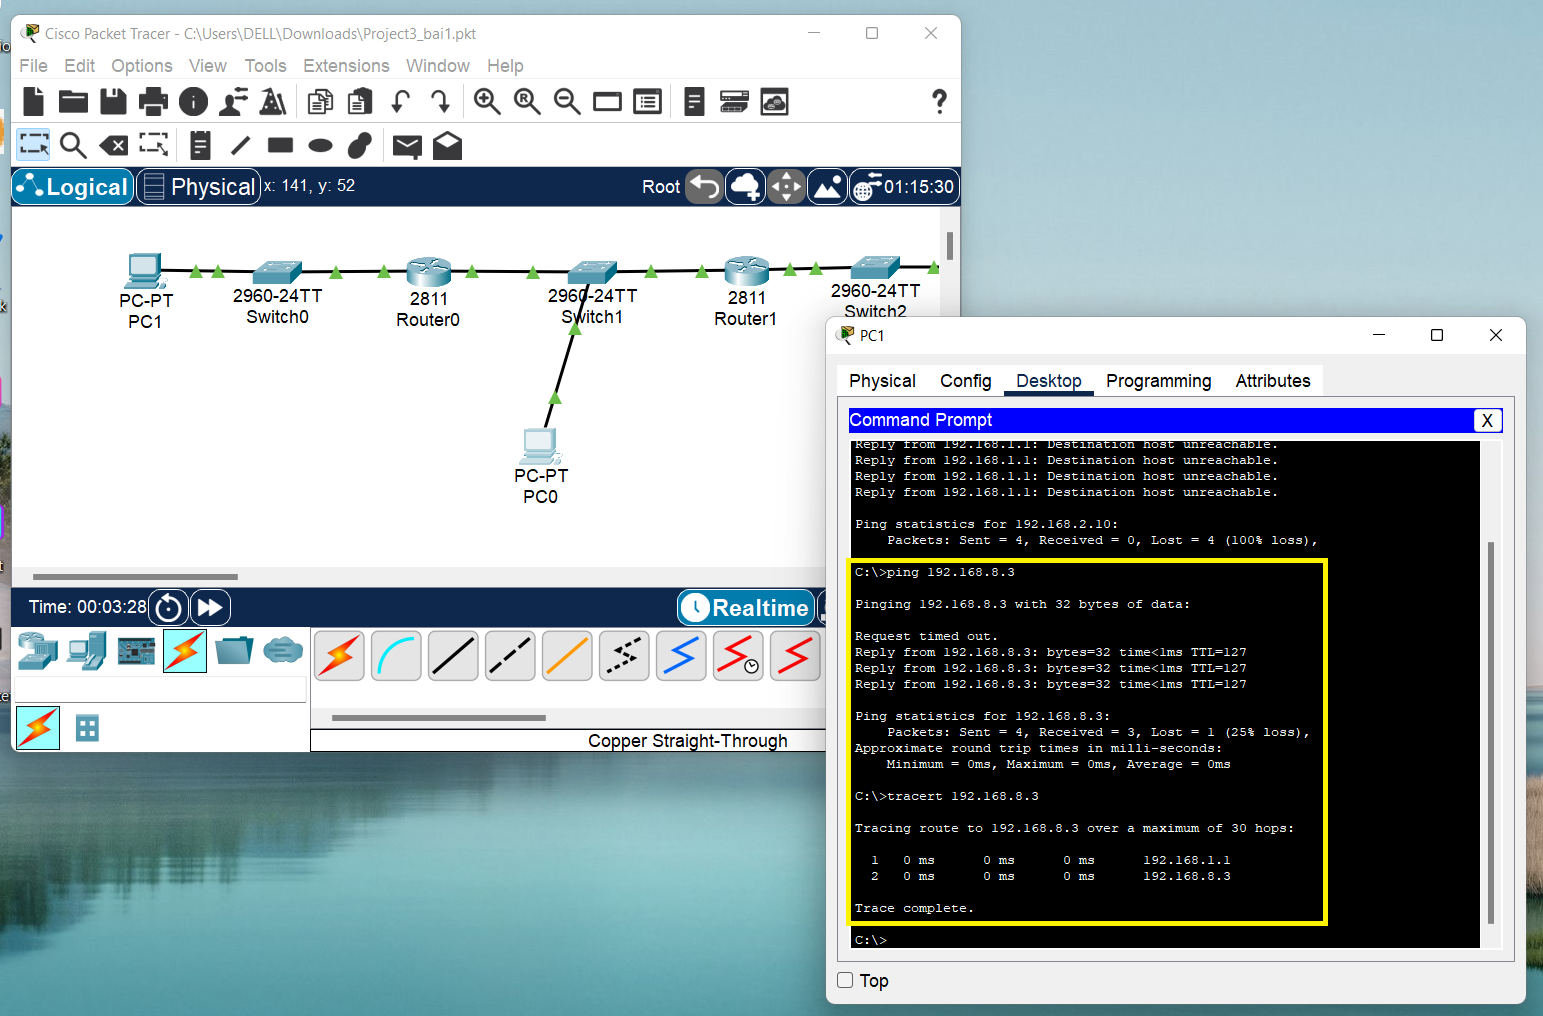
\includegraphics[scale=0.5]{../figures/p1/p1-6}
\end{center}
\caption{Kiểm tra kết nối từ PC0 (\texttt{192.168.1.10}) đến PC2 (\texttt{192.168.8.3})}
\end{figure}

Ở lần \texttt{ping} đầu tiên, có 1 gói tin đầu tiên bị mất, còn lại 3 gói tin kia đều gửi được. Từ lần \texttt{ping} thứ 2, cả 4 gói tin đều gửi được.

Bằng lệnh \texttt{tracert} (hình vẽ) ta thấy được gói tin ICMP đi qua router0, cổng 0: \texttt{192.168.1.1}, sau đó qua cổng 1: \texttt{192.168.8.1} (là default gateway của PC2) đến máy PC2 (\texttt{192.168.8.3}).


\bf \item Thay thế đường default route có trong Router0, Router1 bằng cấu hình định tuyến tĩnh sao cho tất cả các subnet có trong mô hình có thể kết nối lẫn nhau.

\rm Cấu hình static route cho các router:

Click vào router0, mở tab config, vào tab ROUTING/Static, click chuột vào dòng 0.0.0.0/0 via 172.16.1.2 và ấn Remove. Sau đó nhập vào Network 192.168.2.0/24 với Next Hop là 192.168.8.2 và click Add để thêm static route này vào bảng định tuyến. Thực hiện tương tự cho router1.

\begin{figure}[H]
\begin{center}
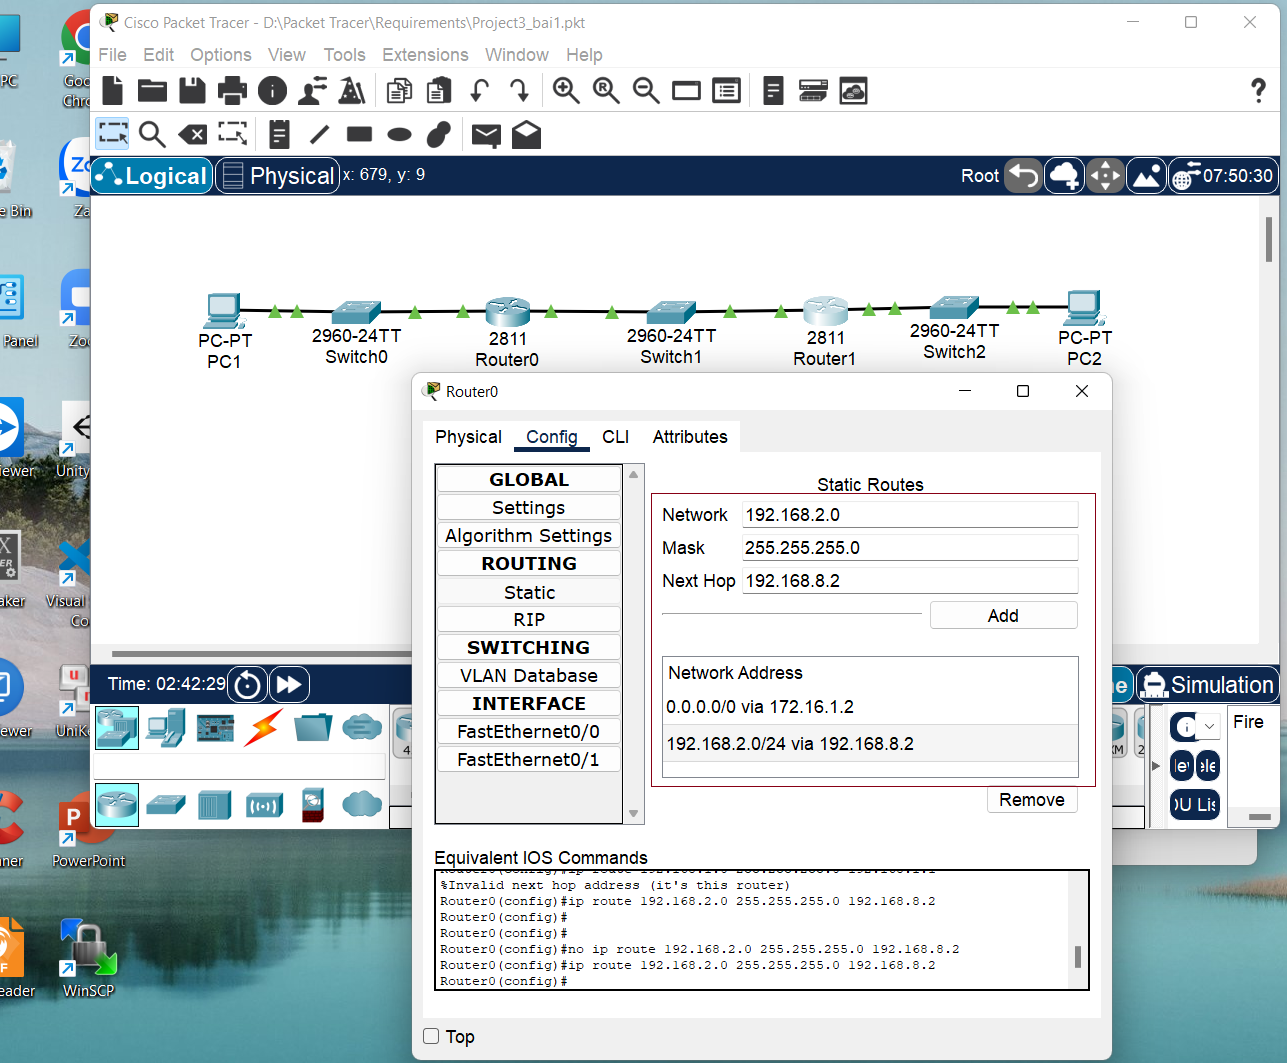
\includegraphics[scale=0.5]{../figures/p1/p1-4a}
\end{center}
\caption{Cấu hình bảng định tuyến cho router0}
\end{figure}

\begin{figure}[H]
\begin{center}
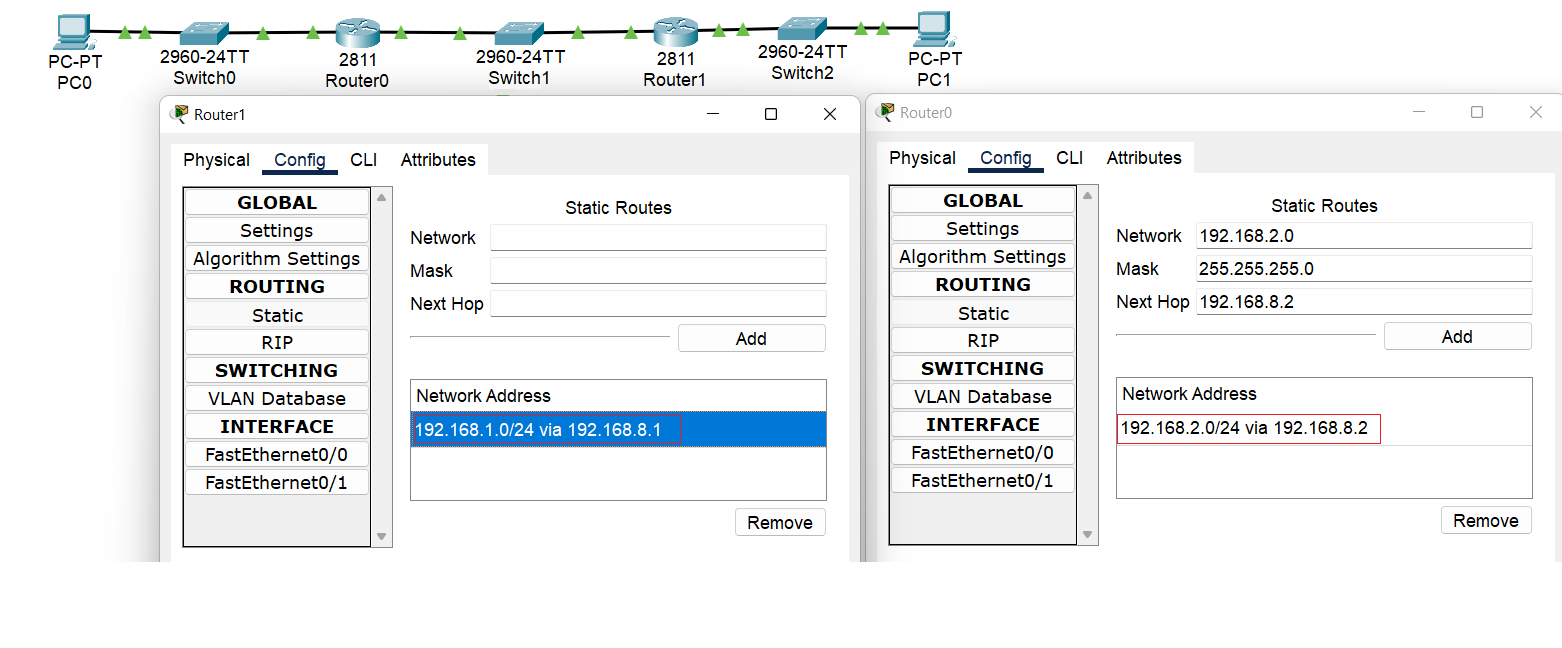
\includegraphics[scale=0.5]{../figures/p1/p1-4b}
\end{center}
\caption{Cấu hình bảng định tuyến cho các router}
\end{figure}

\bf \item Kiểm tra kết nối tất cả các subnet trong mô hình.

\rm Sau khi cấu hình bảng định tuyến cho các router, kết nối được thiết lập, lệnh \texttt{ping} thực hiện được.

\begin{figure}[H]
\begin{center}
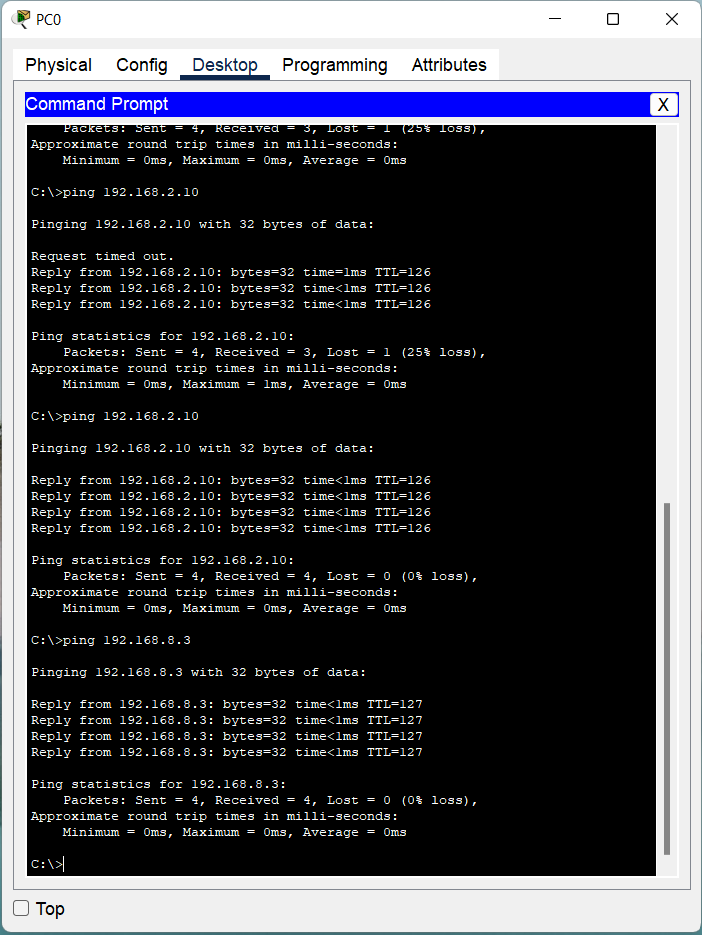
\includegraphics[scale=1]{../figures/p1/p1-70}
\end{center}
\caption{Lệnh \texttt{ping} từ PC0 (\texttt{192.168.1.10}) đến PC1 (\texttt{192.168.2.10}) và PC2 (\texttt{192.168.8.3}) sau khi cấu hình bảng định tuyến tĩnh}
\end{figure}

Lệnh \texttt{ping} từ PC2 sang 2 máy kia:

\begin{figure}[H]
\begin{center}
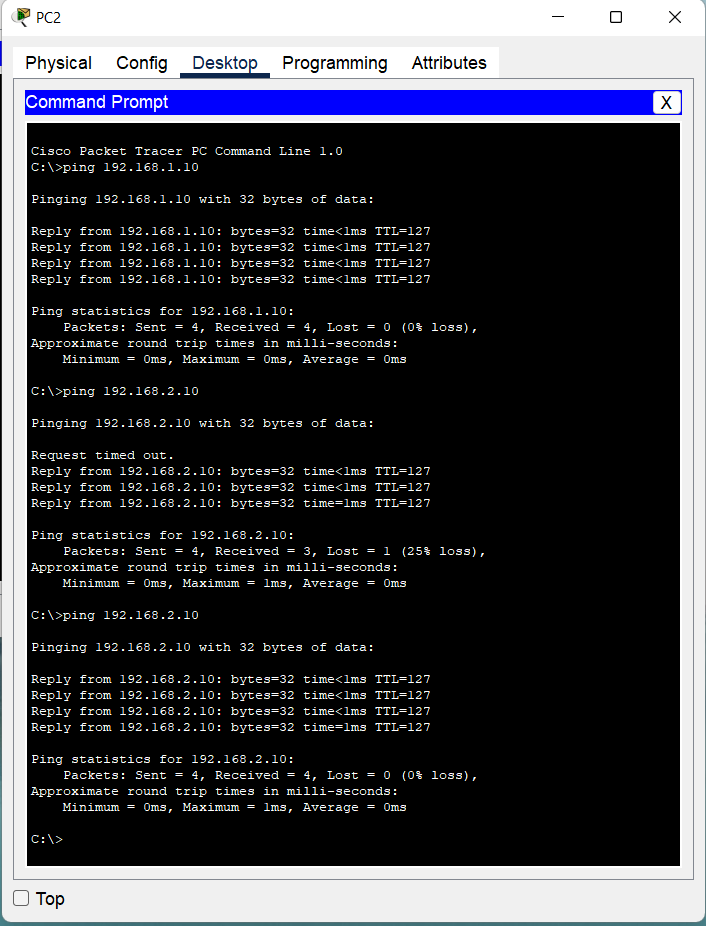
\includegraphics[scale=1]{../figures/p1/p1-72}
\end{center}
\caption{Lệnh \texttt{ping} từ PC2 (\texttt{192.168.8.3}) đến PC0 (\texttt{192.168.1.10}) và PC1 (\texttt{192.168.2.10}) sau khi cấu hình bảng định tuyến tĩnh}
\end{figure}

Lệnh \texttt{ping} từ PC1 sang 2 máy kia:

\begin{figure}[H]
\begin{center}
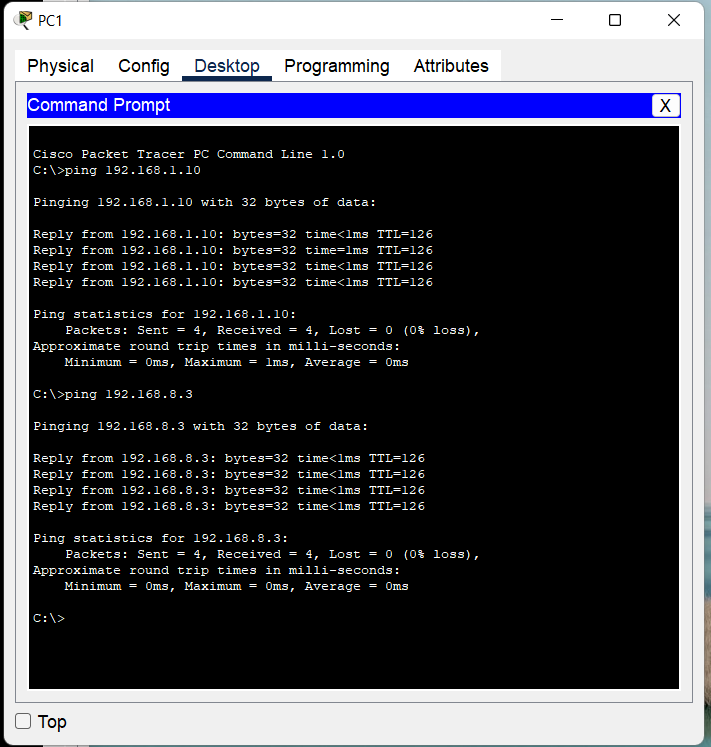
\includegraphics[scale=1]{../figures/p1/p1-71}
\end{center}
\caption{Lệnh \texttt{ping} từ PC1 (\texttt{192.168.2.10}) đến PC0 (\texttt{192.168.1.10}) và PC2 (\texttt{192.168.8.3}) sau khi cấu hình bảng định tuyến tĩnh}
\end{figure}

Kết quả khi kết thúc được lưu trong tập tin \texttt{bai1.pkt}
\end{enumerate}
